%!TEX root = ../thesis.tex

\section{ROS 2}
ROS 2(Robot Operating System versition 2)\cite{ros2}は, オープンソースのロボットソフトウェアフレームワークであり,
ロボットアプリケーションの開発や実行をサポートするミドルウェアである.
異なるバージョンが存在しているが, 本研究ではROS 2 foxyを主に使用している.

\subsection{RViz2}
RViz2(ROS VIsualization 2)\cite{rviz}はROS 2で提供される三次元ビジュアライゼーションツールであり, 
数値で表されるロボットの座標や各センサのデータを視覚的に表すことができる.

\begin{figure}[H]
  \centering
 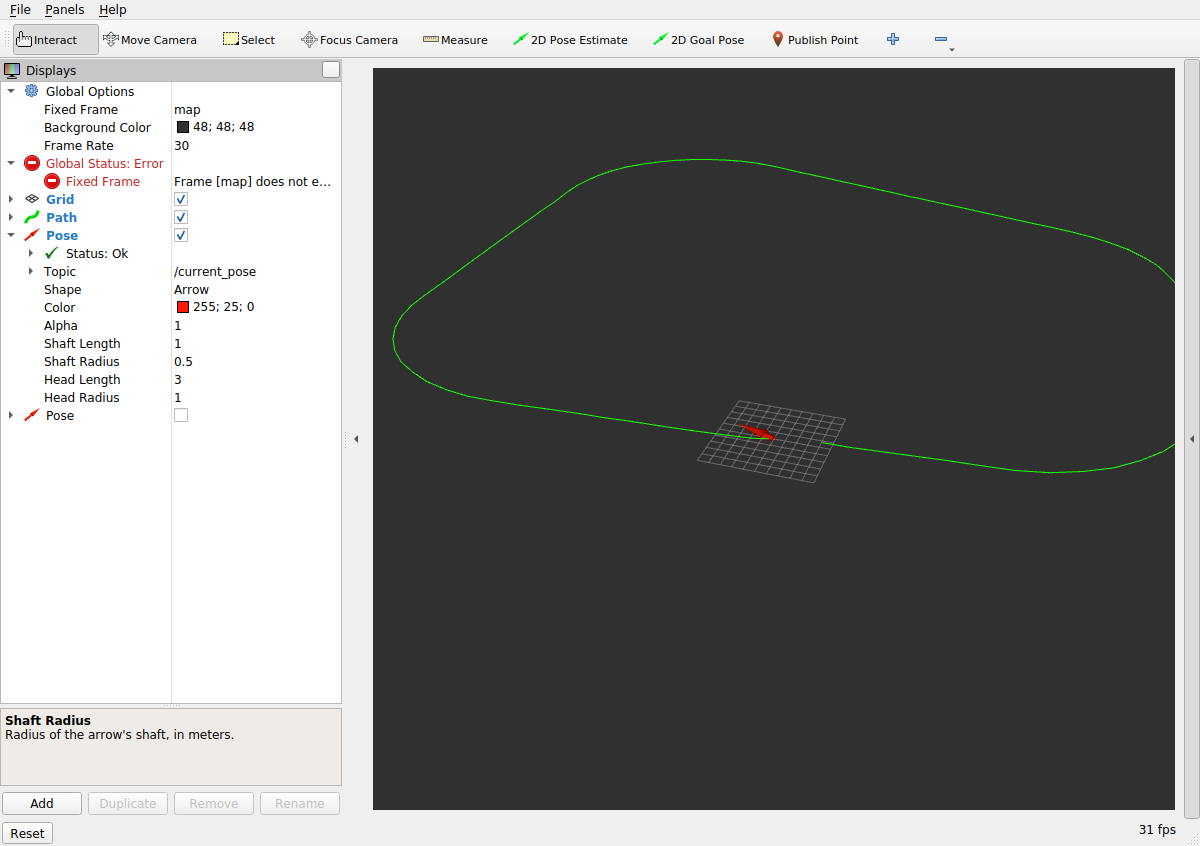
\includegraphics[keepaspectratio, scale=0.4]
     {images/rviz.png}
 \caption{RViz2 view}
 \label{fig:purepursuit}
\end{figure}

\section{GNSS}
GNSS(Global Navigation Satelite System)は, 
人工衛星を利用して地上の現在位置を計測するためのシステムであり, 
アメリカのGPS, ロシアのGLONASS, ヨーロッパのGalileo, 日本のQGSSなどを総称した衛生測位システムを指す.

計測する値は衛生と受信機(アンテナ)間の距離であり, 衛生位置を既知として受信機の三次元座標と受信機時計の誤差を未知数として最低4つの観測値から座標計算される.
測定された距離にはさまざまな誤差要因が含まれる.

\subsection{UTM座標系}
UTM(Universal Transverse Mercator)座標系\cite{utm}とは, 全世界を経度6度ごとのゾーンに分けて東回りに番号を付けて規格化したものである.
世界的にも大・中縮尺の図法として採用され, 日本では国土地理院の地形図や地勢図で採用されている.

\begin{figure}[H]
  \centering
 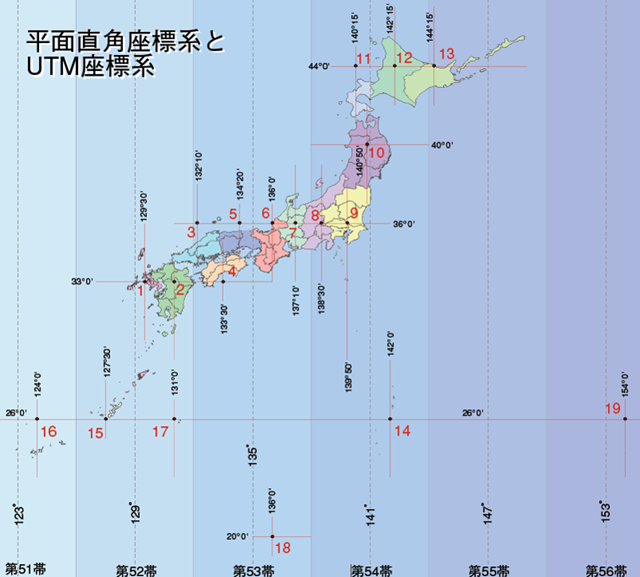
\includegraphics[keepaspectratio, scale=0.7]
      {images/UTMCoordinateSystem.png}
 \caption{UTM Coordinate System(source : [7]}
 \label{fig:UTM}
\end{figure}

% AIFormulaの会場となるAIモビリティパークは茨城県常総市にあるため, 54帯のUTM座標系を使用する.

\subsection{ECEF座標系}
ECEF(Earth-Centered, Earth-Fixed)座標系とは, 地理的・直交的な座標系であり, 地球の自転と同期して常時回転している座標系である.

\subsection{測地座標系}
測地座標系とは, 地球上の位置を緯度, 経度, および回転楕円体からの高さで表す座標系である.

\subsection{マルチパス}
マルチパスとは, 電波がまっすぐに届くだけでなくビルなどの高層建造物に反射して複数のルートを通って伝播することである.
反射した電波は到達するまでにわずかな遅れを生じ, 遅れの時間の分だけ距離が遠いと計測されてしまうため, 正確な測位を乱す要因の一つとなっている.

\begin{figure}[H]
  \centering
 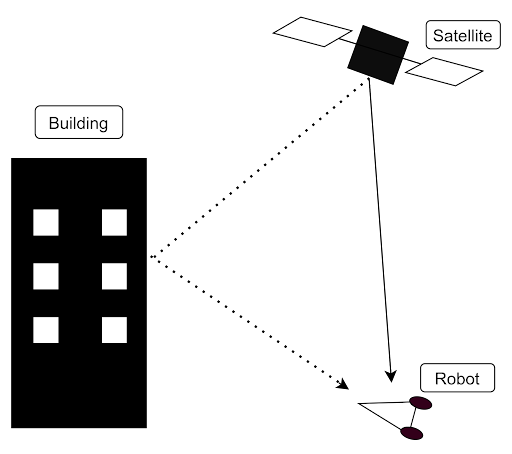
\includegraphics[keepaspectratio, scale=0.4]
      {images/multipath.png}
 \caption{Multipath}
 \label{fig:multipath}
\end{figure}

\section{IMU}
IMU(Inertial Measurement Unit)は, 
3次元の慣性運動を検出する装置である. 
加速度センサーにより並進運動を検出し, 
ジャイロセンサーにより回転運動を検出することができる.

\section{PID制御}
PID制御(Proportional-Integral-Differential Controller)は, 制御工学におけるフィードバック制御の一種である.
出力値と目標値との偏差, その積分, および微分の3つの要素によって, 入力値の制御を行う方法である.

\subsection{P制御}
基本的なフィードバック制御として比例制御(P制御)がある.
これは操作量を制御量と目標値の偏差の一次関数として制御するものである.
PID制御では, この偏差に比例して操作量を変化させる動作を比例動作, またはP動作といい, その時の定数は比例ゲイン, Pゲインと呼ばれる.

\subsection{I制御}
P制御において, 周囲の環境が変わるたびに残留偏差をなくすように比例ゲインを決定しなおすことが難しい.
そこで, 残留偏差が存在する場合, その偏差の時間積分に比例して入力値を変化させる動作をする項を追加する.
追加した項が持つ役割がI制御である.
偏差のある状態が長い時間続けばそれだけ入力値の変化を大きくして目標値に近づけようとする役目を果たす.
ここで, 定数は積分ゲイン, Iゲインと呼ばれる.

\subsection{D制御}
PI制御の問題点として, 周囲の環境が変化したり制御対象に撹乱が加わったりすることで出力値が急に変動することがある.
この問題を解決するために, 急激な出力値の変化が起こった場合, その変化の大きさに比例した入力を行うことでその変化に抵抗する役割を持つ項を追加する.
追加した項が持つ役割がD制御である.
定数は微分ゲイン, Dゲインと呼ばれる.

\newpage